\section{Experimental Results}

\label{sec:experimentalResults}
\subsection{Uncertainty base active learning}
\begin{figure}[!htb]%
    \centering
    \subfloat[]{{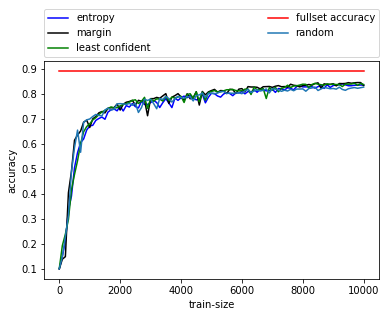
\includegraphics[width=5cm]{Contens/results/confident.png} }}%
    \qquad
    \subfloat[]{{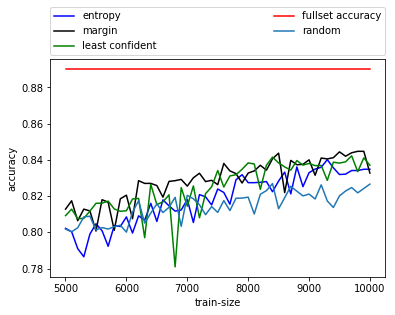
\includegraphics[width=5cm]{Contens/results/confident2.png} }}%
    \caption{Uncertainty base}%
    \label{fig:uncertainty1}%
\end{figure}
\subsection{BALD}

\begin{figure}[!htb]%
    \centering
    \subfloat[]{{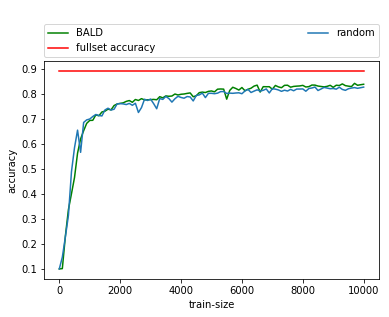
\includegraphics[width=5cm]{Contens/results/Bald1.png} }}%
    \qquad
    \subfloat[]{{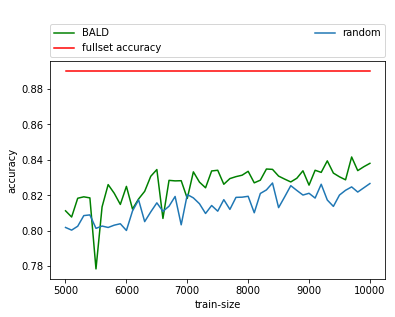
\includegraphics[width=5cm]{Contens/results/Bald2.png}.png} }%
    \caption{BALD}%
    \label{fig:BALD}%
\end{figure}
\subsection{Uncertainty base active learning}

Results should be clearly displayed and should provide a suitable representation of your results for the points you wish to make. Graphs should be labeled in a legible font and if more than one result is displayed on the same graph then these should be clearly marked.   Please choose carefully rather than presenting every results. Too much information is hard to read and often hides the key information you wish to present. Make use of statistical methods when presenting results, where possible to strengthen the results.  Further, the format of the presentation of results should be chosen based on what issues in the results you wish to highlight. You may wish to present a subset in the experimental section and provide additional results in the appendix.
\subsection{Least Confidence }
\subsection{Entropy Sampling}